\documentclass[format=acmsmall, review=false, screen=true]{acmart}

\usepackage[utf8]{inputenc}
\usepackage{booktabs} % For formal tables
\usepackage{subcaption}
\usepackage[capitalise, noabbrev]{cleveref}

\newtheorem{exmp}{Example}[section]

% Copyright
\setcopyright{none}

\settopmatter{printacmref=false} % Removes citation information below abstract
\renewcommand\footnotetextcopyrightpermission[1]{} % removes footnote with conference information in first column
\pagestyle{plain} % removes running headers

\begin{document}
\title{CatBoost applicability in regression problems}

\author{Anna Berger}
\email{a.berger@student.utwente.nl}

\author{Ashwin Sadananda Bhat}
\email{a.sadanandabhat@student.utwente.nl}


% The default list of authors is too long for headers.

\begin{abstract}
Gradient boosting is one of the rapidly developing and widely used techniques which is acknowledged to be a powerful tool in both industrial problems and machine learning competitions. A recently appeared library CatBoost for gradient boosting on decision trees is claimed to outperform existing implementations by special processing of categorical variables and improved process of gradient estimation. It is claimed to outperform existing state-of-the-art models on several benchmarks for classification with no regards to any regression problems. This paper investigates the applicability of CatBoost  in the regression problem of housing price prediction. We compare its performance with the performance of two other gradient boosting libraries such as sklearn and XGBoost by training and evaluating them on three datasets with different properties. We also analyze categorical feature importance and their influence on performance.
\end{abstract}


\maketitle
\thispagestyle{plain}


\begin{frame}{Gradient Boosting: what is it?}
	\begin{figure}
		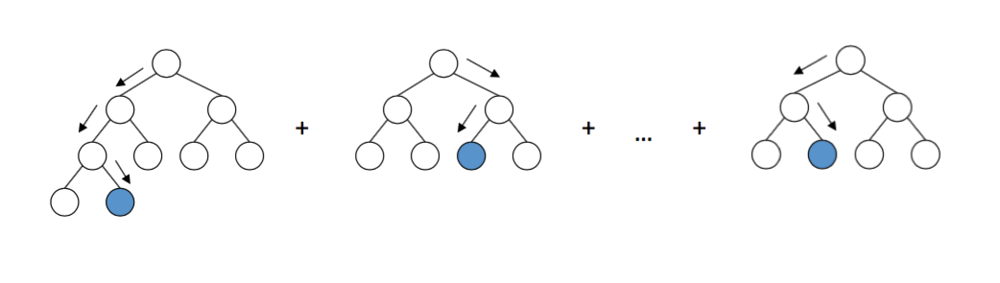
\includegraphics[width=\textwidth]{figures/gbdt}
	\end{figure}
\end{frame}

\begin{frame}{Gradient Boosting: libraries}
	\begin{columns}
		\begin{column}{0.33\textwidth}
			\centering
			\begin{figure}
				
\includegraphics[width=\columnwidth]{figures/scikit}
			\end{figure}
		\end{column}

		
		\begin{column}{0.33\textwidth}
			\centering
			\begin{figure}
				
\includegraphics[width=\columnwidth]{figures/catboost}
			\end{figure}
		\end{column}
		
		\begin{column}{0.33\textwidth}
			\centering
			\begin{figure}
				
\includegraphics[width=\columnwidth]{figures/xgboost}
			\end{figure}
		\end{column}
		
	\end{columns}
\end{frame}

\begin{frame}{Research question}
	
\end{frame}

\begin{frame}{Related work}
	\begin{enumerate}
		\item[\textbf{[1]}] Tianqi Chen and Carlos Guestrin. 2016. XGBoost: A Scalable Tree Boosting System. 
		\item[\textbf{[2]}] Anna Veronika Dorogush, Vasily Ershov, Andrey Gulin. 2017. CatBoost: gradient boosting with categorical features support
	\end{enumerate}
\end{frame}

\begin{frame}{Data}
	3 datasets (Kaggle):
	\begin{enumerate}
		\item Sberbank Russian Housing Market dataset 
		\item Ames Housing dataset 
		\item Boston Housing dataset 
	\end{enumerate}
\end{frame}

\section{Related Work}
\label{sec:related-work}

To the best of our knowledge, the paper written by \citet{breiman1997arcing}  is one of the earliest in the GBDT field. It comprises the idea of viewing gradient boosting as the optimization algorithm minimizing certain cost function. This concept was subsequently developed by \citet{friedman2001greedy} who proposed to make the connection between stagewise model expansions and steepest-descent minimization and to consider boosting algorithms as iterative functional gradient descent algorithms. The intuition behind that work is that function minimization can be performed by repeatedly adding an imperfect model pointing to the direction of negative gradient to the existing one so as to correct the errors of the predecessors.

The gradient boosting is frequently used with decision trees as base functions. To determine the next base predictor, the enumeration of all possible splits on all the features has to be performed. The GBDT implementation provided by scikit-learn \cite{scikit-learn} employs exact greedy algorithm for choosing the predictor contributing the greatest score improvement. Since complete enumeration is computationally demanding, \citet{chen2016xgboost} propose an implementation called XGBoost which comprises an approximate algorithm for enumerating all possible splits in continuous features and several system design optimizations. These improvements allow to create a well-scalable model which outperforms the models existing by that time together with significant training process speed-up.

One of the most recent studies by \citet{DBLP:journals/corr/DorogushGGKPV17}, \cite{dorogushcatboost} proposes a new gradient-boosting library CatBoost which incorporates information contained in categorical features establishing a new strategy of computing the statistics for the category labels. Another crucial enhancement is a new way of 
identifying and solving a bias problem in pointwise gradient estimates which is present in classical boosting algorithms and their existing implementations. Proposed implementation outperforms the existing libraries in terms of prediction quality on several benchmarks in classification tasks without any regards to regression problems which served us a motivation to perform a research in this particular area.
\section{Data}
\label{sec:data}
Throughout this project we make use of three datasets for housing price prediction publicly available from Kaggle competitions. We choose them under assumption that testing the GBDT models on various datasets with distinctive properties is important for reasoning about their performance in housing price prediction area. 

The first dataset we utilize is a classic but tiny Boston dataset \cite{boston1978housing} collected in 70's. It encloses 333 instances described by 13 features, only one of which is categorical in itself. Despite the modest size this dataset can still be employed as a rapid and reasonable initial step towards understanding of model's performance in regression problems.

We also adopt the Ames housing dataset \cite{de2011ames} incorporating 1460 observations and 80 explanatory variables involved in assessing home price: 43 categorical and 37 ordinal and continuous. It describes the sale of individual residential property in Ames, Iowa from 2006 to 2010 and includes much greater variety of information than the Boston dataset.

The third dataset is provided by Russian bank Sberbank \cite{sberbank2017housing} and not only includes housing specifications but also comprises macroeconomic patterns. It contains 12231 training instances each of which represented by 293 parameters with 18 categorical among them. This dataset is the most diverse among all the considered datasets which imposes a significant challenge to the models.

Comparative analysis shows that the Ames housing dataset offers the greatest variety of categorical features which are of the most interest taking into account specific CatBoost treatment towards them. The Sberbank dataset seems to be the most appealing in the sense of being true to life as it is mostly collected by the real estate companies which, on the other hand, makes it more noisy, and therefore, more demanding for model training.
\section{Methodology}
\label{sec:methodology}

This section briefly explains the main differences of CatBoost library from the wide-spread industrial gradient boosting implementations such as scikit-learn and XGBoost. Furthermore, we discuss performed data preprocessing and the evaluating procedure.

\subsection{Model}

In our research we compare the performance of CatBoostRegressor from CatBoost library with other two existing publicly available implementations of gradient boosting algorithm for regression problems: GradientBoostingRegressor from scikit-learn and XGBoostRegressor from XGBoost. There are two fundamental key points which we consider remarkable in the CatBoost implementation.

Firstly, it adopts an efficient strategy for handling categorical features in the data which is essentially substituting the category labels with some statistics computed per category with incorporated intention of prevented overfitting. To accomplish this, it performs a random permutation of the dataset and for each example it computes average label value for the example with the same category value placed before the given one in the permutation. 
If we denote the permutation as $ \sigma = (\sigma_1, ..., \sigma_n)$, the feature vector as $ X_i = (x_{i, 1}, ..., x_{i, n})$, the label value as $Y_i$ and the prior value with its weight as $P$ and $a$ respectively then the statistics is computed by the following formula:

$$ \frac{\sum_{j=1}^{p-1} [ x_{\sigma_j, i} = x_{\sigma_p, i}] Y_{\sigma_j} + a \cdot P}{\sum_{j=1}^{p-1} [ x_{\sigma_j, i} = x_{\sigma_p, i}] + a }. $$

Adding the prior helps reducing the noise obtained from low-frequency categories. The standard technique for choosing the prior in regression problems is to take the average label value in the dataset.

Secondly, CatBoost suggests a principled way of mitigating the problem of biased pointwise gradient estimates and proposes dynamic boosting approach that avoids the estimation bias at a minimal cost of the variance of the gradient estimation. Usually gradients on each iteration are assessed using the same data points which leads to a shift from actual distribution of gradients in any domain in the feature space. To overcome this problem, for each training instance a separate model is employed which is never updated using the gradient estimate for this example. CatBoost implementation follows one relaxation of this idea which makes it feasible to employ: all these separate models share the same tree structures. TODO

\subsection{Training}

In this project we examine the performance of three classifiers, namely GradientBoostingRegressor from scikit-learn, XGBoostRegressor from XGBoost and CatBoostRegressor from CatBoost. We assess the performance of these models in the field of housing price prediction by applying them on three different datasets described in \cref{sec:data} without any preliminary feature selection as we do not opt for gaining the highest but for analyzing models conduct in the same conditions.

In order to make use of GradientBoostingRegressor we first need to preprocess the data: for numerical columns we replace the missing values with the mean along each column whereas for categorical variables we perform one-hot encoding. Regarding XGBoostRegressor, we solely rely on its internal missing values treatment but repeat the procedure of binarizing the categorical variables. We do not adopt any additional feature preprocessing for CatBoostRegressor, only explicitly specify the categorical variables for its further internal processing. All the models are first trained with their default parameters which one can find in Appendix \cref{tab:default-parameters} and later tuned by employing the grid search over the predefined set of parameters which can be found in Appendix \cref{tab:grid-search-parameters}.

\subsection{Evaluation}

To evaluate the regression problem we employ the Root Mean Squared Logarithmic Error (RMSLE) as it equally penalizes the mismatches within small and huge values. Let $p_i$ be the predicted values and $a_i$ the actual values, then RMSLE is computed as follows:

$$ RMSLE = \sqrt[]{\frac{1}{N}\sum_{n = 1}^N (\log(p_i + 1) - \log(a_i + 1))^2}. $$

In order to assess the performance of the discussed algorithms and perform the grid search, we employ 5-fold cross validation. Throughout this research, the training speed is also of great interest for us, and thus, we measure the training time 3 times in a row and report the average of them.




\section{Results}
\label{sec:results}
This section discusses the experimental results of this project. We present the RMSLE scores for both default and tuned models when cross-validated on each of three datasets together with the training time taken.  

\subsection{Sberbank Dataset}
From our perspective, this dataset can be called the most challenging among the observed ones but at the same time the most practice-oriented as it comprises substantial amount of information incorporated in 293 features and more than 12000 features. As can be seen from \cref{tab:sberbank-results}, the performance of all three models is very similar for both default and tuned models, although XGBoost slightly outperforms the others. However, they significantly differ in the terms of training time: CatBoost is more than four times slower than two other models. 

\begin{table}[htbp]
	\centering
	\resizebox{\linewidth}{!}{
		\begin{tabular}{lrrrr}
			\toprule
			\textbf{Model} & \textbf{Default} & \textbf{Tuned} & \textbf{Best: depth, estimators, learning rate} & \textbf{Training time} \\
			\midrule
			CatBoost & 0.5161 &  0.5102 & 3, 100, 0.01 & 765.91 \\
			XGBoost & \textbf{0.5098} & \textbf{0.5081} & 2, 500, 0.05 & 158.67 \\
			sklearn GB & 0.5102 & 0.5091 & 1, 1000, 0.1  & \textbf{148.41} \\
			\bottomrule
		\end{tabular}
	}
	\caption{Sberbank dataset results}
	\label{tab:sberbank-results}
\end{table}

\subsection{Ames Dataset}
\cref{tab:ames-results} presents the results obtained when training the models on Ames dataset. Examining it, we can derive that sklearn GB and XGBoost do comparably well with CatBoost slightly lagging behind for both the default and tuned models. We expected CatBoost to outperform the other models on this dataset as more than a half of its features are categorical. However, special processing of categorical features does not result in the substantial performance gain.

\begin{table}[htbp]
	\centering
	\begin{tabular}{lrrrr}
		\toprule
		\textbf{Model} & \textbf{Default} & \textbf{Tuned} & \textbf{Best: depth, estimators, learning rate} & \textbf{Training time}  \\
		\midrule
		CatBoost & 0.1789 &  0.1435 & 1, 1000, 0.1  & 58.82\\
		XGBoost & 0.1315 & 0.1246 & 2, 500, 0.1 & \textbf{8.72} \\
		sklearn GB & \textbf{0.1285} & \textbf{0.1241} & 1, 1000, 0.1 & 10.10 \\
		\bottomrule
	\end{tabular}
	\caption{Results on the Ames dataset}
	\label{tab:ames-results}
\end{table}

\subsection{Boston Dataset}
It can be observed from the results for Boston dataset given in \cref{tab:boston-results} that it is the only dataset on which CatBoost succeeds to outperform other GDBT implemenations. However, this slight advantage gained in performance comes at the cost of training time taken: XGBoost is approximately 75 times faster than CatBoost and sklearn GB is 52 times faster than CatBoost. 

\begin{table}[htbp]
	\centering
	\begin{tabular}{lrrrr}
		\toprule
		\textbf{Model} & \textbf{Default} & \textbf{Tuned} & \textbf{Best parameters} & \textbf{Training time}  \\
		\midrule
		CatBoost & \textbf{0.1584} &  \textbf{0.1423} & 1, 1000, 0.01  & 56.33 \\
		XGBoost & 0.1952 & 0.1753  & 2, 1000, 0.01  & \textbf{0.75} \\
		sklearn GB & 0.1993 & 0.1721 & 2, 1000, 0.01  & 1.07 \\
		\bottomrule
	\end{tabular}
    \caption{Results on the Boston dataset}
	\label{tab:boston-results}
\end{table}




\section{Discussion}
\label{sec:discussion}
It has been observed throughout the experiments that all three models show rather similar performance on the housing price datasets under consideration. In order to investigate the contribution of categorical variables into making the final decision we explore the feature importances provided by each of the GBDT implementations. Feature importance reflects the  informativeness of the characteristic for the model. It is computed as the normalized total reduction of the criterion brought by that feature and is also known as the Gini importance. We examine the number of categorical variables in the top 10 most important features for each model and summarize the observations in \cref{tab:feature-importance}.

\begin{table}[htbp]
	\centering
	\resizebox{0.7\linewidth}{!}{
		\begin{tabular}{lrrr}
			\toprule
			\textbf{Model} & \textbf{Russia} & \textbf{Ames} & \textbf{Boston} \\
			\midrule
			CatBoost & 5& 9 & 1 \\
			XGBoost & 1  & 1 & 0 \\
			sklearn & 1 & 0 & 0 \\
			\midrule
			\textbf{Number of categorical features} & 18 & 43 & 1 \\
			\textbf{Total number of features} & 293 & 80 & 13 \\
			\bottomrule
		\end{tabular}
	}
	\caption{Number of categorical features among top 10 most important for the model }
	\label{tab:feature-importance}
\end{table}

As can be seen from \cref{tab:feature-importance}, CatBoost gives clear precedence to the categorical variables whereas other models do not demonstrate any particular preference for them. We assume that this is due to the sophisticated encoding of categorical variables provided by the CatBoost. However, this special treatment does not necessarily boost the performance whereas seriously increasing the training time as we could perceive from \cref{sec:results}. 

With respect to the encountered experience of applying CatBoost to the housing price prediction task, we see that it obtains sufficient results when compared to other state-of-the-art models. However, it does not consistently outperform them and one possible reason for this can be its still imperfect optimization for regression problems which would also explain the absence of information regarding its performance on regression tasks. Another prominent problem that we came across is long training time of this model which prevented us from performing more extensive grid search. It is conceivable that with more training resources we could have gained better score for CatBoost as apparently, it incorporates elaborate approaches towards categorical variable processing and building weak estimators which require much more computational power that we has at our disposal. However, it is an open question whether several percent improvements are worth significant training time consuming.
\section{Conclusion}
\label{sec:conclusion}

In this research we investigate the applicability of a recently appeared new implementation of GDBTs CatBoost with inbuilt intricate categorical feature preprocessing and advanced approach to fighting the bias in gradient estimation. We employ two more competitive GBDT implementations and compare their performance of three different datasets for housing price prediction. During the research, we found out that CatBoost outperforms two models only on the smallest dataset with the smallest number of features while still deferring to them in more realistic dataset. Further analysis shows its apparent preference towards the categorical variables while building the solution.

In case we would have more time and additional resources, we would firstly employ the GPU version of the CatBoost library which could gain additional score improvement taking into account long training time which prevented us from fully exploring all the powers of this library. Also it can be beneficial for all three libraries to explore smaller feature subsets as for close-to-life datasets they are really sparse which introduces much noise in the data and can be one of possible reasons of errors. Finally, it would be interesting to extend this research to other regression problems providing more general approach to this problem without focusing on specific things which are typical to house price prediction area.

\bibliographystyle{ACM-Reference-Format}
\bibliography{bibliography} 

\appendix
\section{Supplemental Materials}



\end{document}
